\section {Rezultate experimentale}

\paragraph{}
Av'and definite re'telele de tip ANFIS 'si cunosc'and acum modelul COCOMO, reamintim scopul experimentului: predic'tia efortului dezvolt;arii unui proiect software plec'and de la factorii de cost COCOMO 'si estimarea proiectului 'in mii de linii de cod surs;a livrate. 
\par
\subsection{Metodologia de lucru}
Datele pe care le-am folosit au fost prezentate 'in capitolul 4. Acestea au fost 'imp;ar'tite, 'in mod randomizat, 'in 85\% date de antrenare 'si 15\% date de testare. Urm;atorul pas a fost aplicarea normaliz;arii min-max peste acestea, astfel 'inc'at valorile extreme s;a nu aib;a o pondere exagerat;a fa't;a de restul datelor.
\begin{figure}[!htbp]
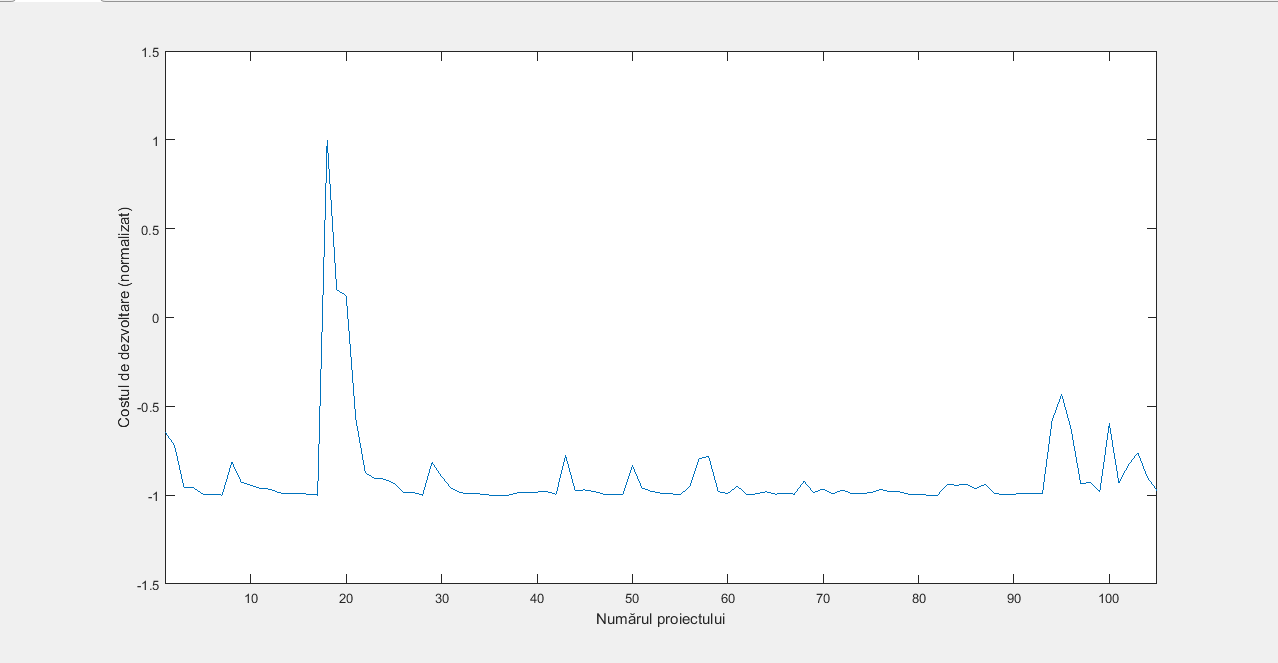
\includegraphics[width=\textwidth]{training_cost}
\caption{Reparti'tia costurilor din mul'timea de antrenare pentru fiecare proiect}
\end{figure}
\par
Putem observa u'sor din Figura 9.1 c;a exist;a valori extreme 'in date, astfel justific'and normalizarea datelor.
\par
Odat;a normalizate datele am creat un sistem de inferen't;a fuzzy pentru datele de intrare, folosind algoritmul de clustering subtractiv, cu valorile 0.8 pentru "Cluster Influence Range", 0.4 pentru "Squash Factor", 0.2 pentru "Accept Ratio" 'si 0.07 pentru "Reject Ratio". Astfel s-a ob'tinut un sistem de inferen't;a fuzzy cu 64 de clustere, fiecare cu c'ate 16 reguli de apartenen't;a pe antecedent.
\par
Sistemul de inferen't;a fuzzy a fost antrenat folosind algoritmul ANFIS pentru 100 de epoci, astfel ajung'and s;a ob'tin;a o eroare RMSE de 'inv;a'tare de 0.0008. Eroarea MMRE este de 0.000270 peste mul'timea de antrenare. Rezultatele pot fi vizualizate 'in figura 9.2.
\newpage
\begin{figure}[!htbp]
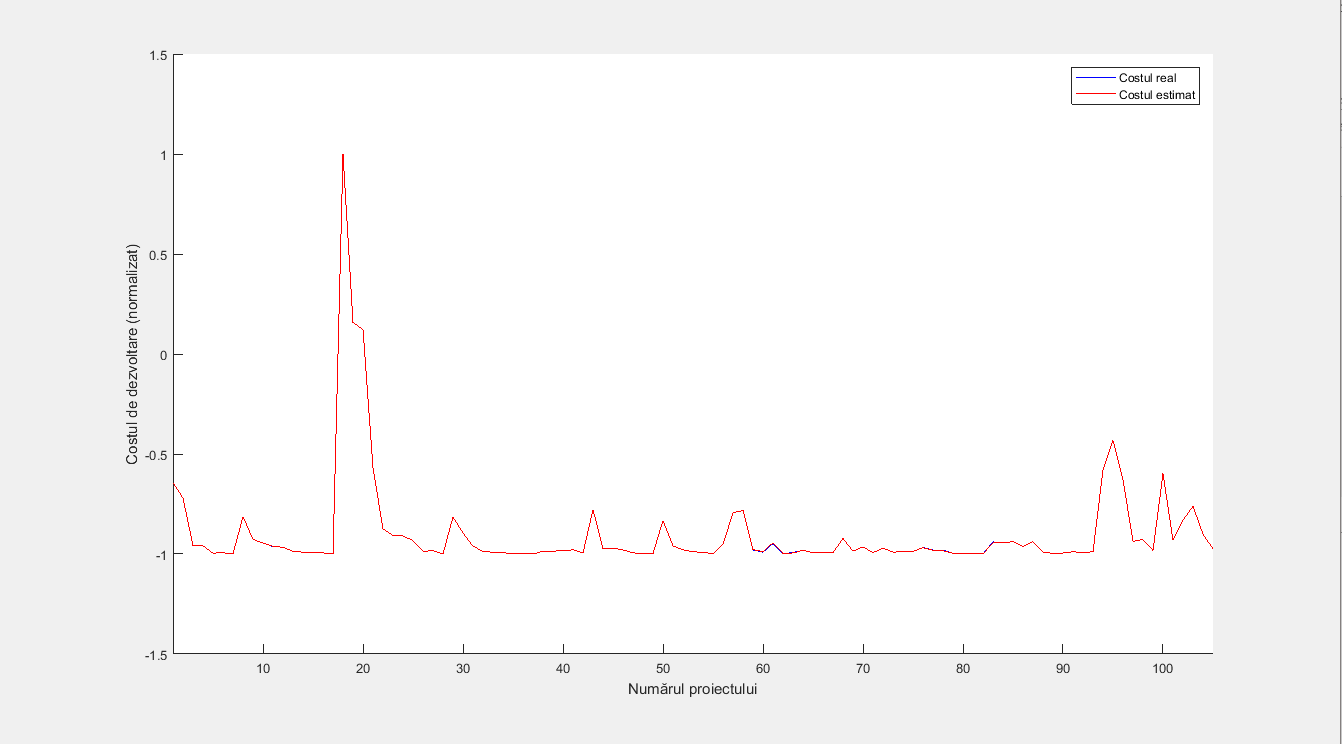
\includegraphics[width=\textwidth]{training_estimated}
\caption{Rezultatele antren;arii vs valorile reale}
\end{figure}
\par
Putem observa o 'inv;a'tare aproape complet;a a datelor de antrenare. Acest lucru nu este neap;arat dezirabil, fiind un indicator c;a modelul sufer;a de overfitting. Ne vom pronun;ta asupra acestui lucru dup;a observarea comportamentului peste datele de testare.
\subsection{Rezultatele evalu;arii re'telei}
P;astr'and re'teaua antrenat;a mai devreme, o vom supune simul;arii peste cele 18 puncte de test pe care le avem la dispozi'tie. 
\par
Rezultatele evalu;arii sunt urm'atoarele:
\begin{itemize}
\item O eroare RMSE de 0.059
\item O eroare MMRE de 0.036
\item O estimare PRED(25) de 1
\end{itemize}
Astfel, este evident c;a fenomenul de overfitting nu a avut loc, sau dac;a acesta a ap;arut se manifest;a insesizabil. Prin urmare, consider;am c;a modelul propus ne ofer;a o rat;a de 'inv;a'tare foarte bun;a, fiind capabil s;a ofere predic'tii cu acurate'te foarte bun;a pentru proiectele modelate sub COCOMO.
\newpage
\begin{figure}[!htbp]
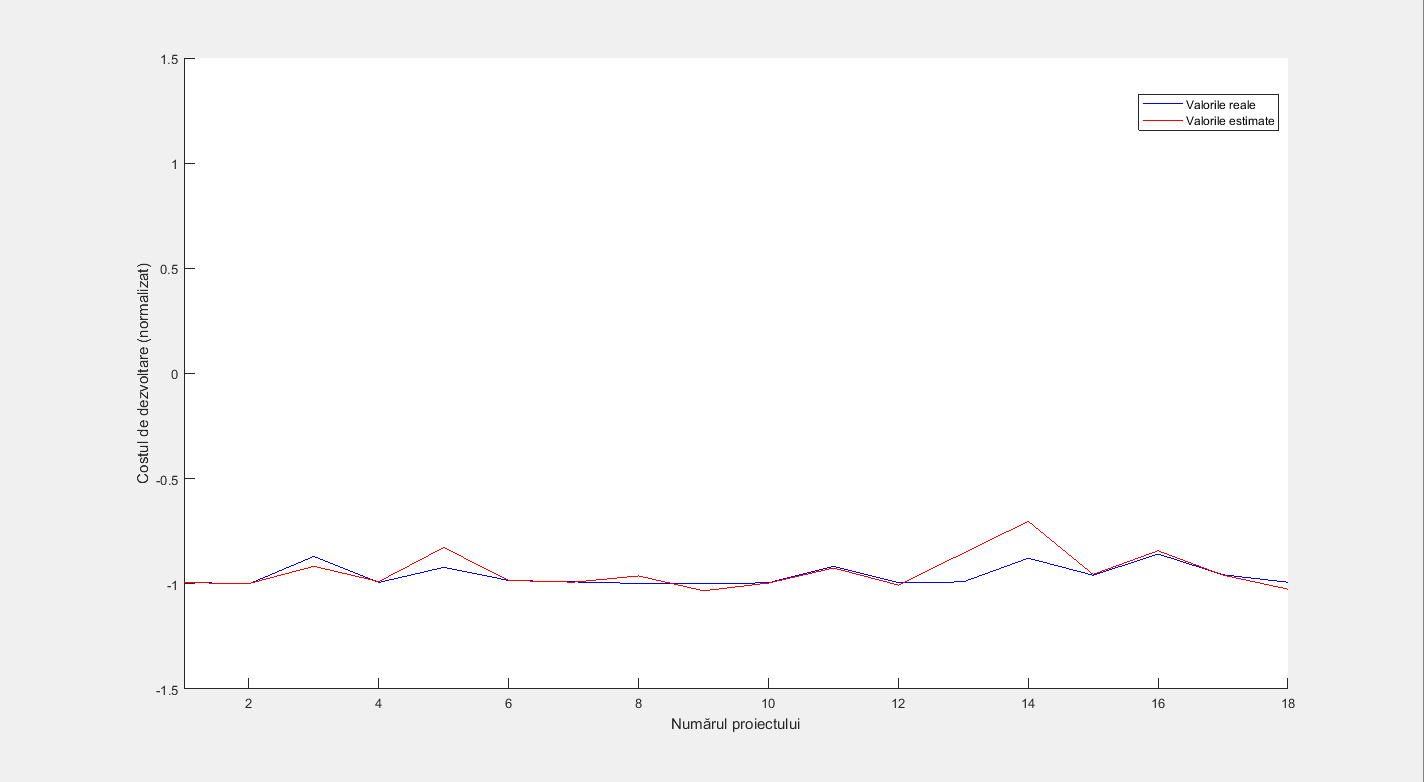
\includegraphics[width=\textwidth]{testing_output}
\caption {Rezultatele evalu;arii datelor de test vs valorile reale}
\end{figure}